\documentclass[10pt]{article}

\def\Type{LessonCaelan}
\def\TypeNum{Lesson 20}
\def\TypeTitle{Intro to Probability and Discrete Random Variables }
\def\Semester{Fall 2021} %Not Used 
\def\Course{MATH 1190 \& 1210}

\usepackage{preambleDJ}



%%%%%%%%%%%% BEGIN DOCUMENT %%%%%%%%%%%%%%%
%%%%%%%%%%%% BEGIN DOCUMENT %%%%%%%%%%%%%%%
%%%%%%%%%%%% BEGIN DOCUMENT %%%%%%%%%%%%%%%
%%%%%%%%%%%% BEGIN DOCUMENT %%%%%%%%%%%%%%%
%%%%%%%%%%%% BEGIN DOCUMENT %%%%%%%%%%%%%%%

\begin{document}


\thispagestyle{firstpage}
\pagestyle{otherpages}
\vs{0.5}



\textbf{Intended Learning Outcomes}
After this lesson, you will be able to 

\begin{itemize}
    \item List outcomes in the sample space or an event of a random process. (\target{P1})
    \item Determine if a random variable is discrete.(\target{P1})
    \item Find a probability of an event when the sample space is finite. (\target{P1})
    %\item Use summations to find the probability that an event modeled by a discrete random variable occurs. (\target{P1})
    \item Determine and use the probability mass function and its properties of a discrete random variable. (\target{P1})
    \item Sketch the histogram representing a probability mass function. (\target{P1})
\end{itemize}

\vspace{-0.5cm}

\hrulefill

\vspace{0.2cm}

\fbox{
\begin{minipage}{0.95\textwidth}
Fill in the blanks.
\begin{itemize}
\item An \rule[-8pt]{1.2in}{0.4pt} is a process that can be infinitely repeated by which we observe something uncertain.

\item An \rule[-8pt]{1.2in}{0.4pt} is a result of one iteration of an experiment. 

\item The \rule[-8pt]{1.2in}{0.4pt} of a random process is the collection of all its possible outcomes.

\item An \rule[-8pt]{1.2in}{0.4pt} is a collection of outcomes from the sample space.
\end{itemize}
\end{minipage}
}

\exercise{\bf\color{Orange}P1} An opaque bag contains 1 {\color{red}red} marble, 1 {\color{ForestGreen}green} marble, and 1 {\color{blue}blue} marble. ({\it Hint:} For example, denote outcomes using notation like {\color{red}R}, {\color{ForestGreen}G}, or {\color{blue}B}, as appropriate!)
    \begin{itemize}
    \item[(a)] In an experiment where one marble is drawn randomly from the bag and the color of the marble is recorded, what is the sample space $S$?

    {\Large
    \[
    S = \rule[-8pt]{4in}{0.4pt}
    \]
    }

    \item[(b)] In another experiment, one marble is drawn randomly from the bag, the color of the marble is recorded, the marble is placed back in the bag, and then a second marble is drawn, its color recorded, and then the marble is placed back in the bag. What is the sample space $S$? ({\bf Note:} we call this drawing {\bf with replacement}.)

    {\Large
    \[
    S = \rule[-8pt]{4in}{0.4pt}
    \]
    }

    \item[(c)] In another experiment, one marble is drawn randomly from the bag, the color of the marble is recorded, the marble is NOT placed back in the bag, and then a second marble is drawn, its color recorded, and then the marble is NOT placed back in the bag. What is the sample space $S$? ({\bf Note:} we call this drawing {\bf without replacement}.)

    {\Large
    \[
    S = \rule[-8pt]{4in}{0.4pt}
    \]
    }
    
    \end{itemize}

%%%%%%%%%
\newpage%
%%%%%%%%%

{\bf Discrete Random Variables and Probabilities of Events}\\

\fbox{

\begin{minipage}{0.95\textwidth}
\begin{itemize}
    \item A \rule[-8pt]{2in}{0.4pt} assigns a number (not necessarily unique) to each outcome in a sample space.
    \item A \rule[-8pt]{2in}{0.4pt} is a random variable that can only take on a finite number of values.
\item When all outcomes in the sample space $S$ are equally likely, then the probability of an event $E$, denoted as $P(E)$, can be computed as:

\[ P(E) = \dfrac{\text{size of the event}}{\text{size of the sample space}} \]

\item For a discrete random variable $X$, the {\bf probability mass function} (PMF) $p(x)$ of the random variable $X$ describes the probabilities that $X$ takes on different values. Generally speaking, $p(x)=P(X=x)$.

\item There are two important properties of probability mass functions.
\begin{itemize}
    \item Each probability in the table must be between \rule[-8pt]{1in}{0.4pt} and \rule[-8pt]{1in}{0.4pt}.
    \item The sum of all probabilities in the table must equal to \rule[-8pt]{1in}{0.4pt}.
\end{itemize}

\item A \textbf{histogram} is a bar graph that visually represents the probability mass function of a discrete random variable. The horizontal axis lists all possible values of the discrete random variable. A bar is created for each possible value where the height of the bar is the probability of this value occurring.

\end{itemize}

\end{minipage}
}

\example{\bf\color{Orange}P1} Let's re-consider the experiment in Exercise A (c). Suppose $X$ is a discrete random variable where $X=0$ represents the event that neither of the two drawn marbles is blue, and $X=1$ represents the event that one of the marbles drawn is blue.

\begin{enumerate}[label=(\alph*)]
    \item Find $P(X=0)$ and $P(X=1)$.

    \vfill

    \item Sketch a histogram representing this probability mass function.

    \begin{center}
    \begin{tikzpicture}[scale=1.25]
          \begin{axis}[
            %xlabel={$x$},
            %grid = major,
            %xtick       = {1,2,3,4,5,6,7,8,9},
            %xticklabels = {$1$,$2$,$3$,$4$,$5$,$6$,$7$,$8$,$9$},
            %ytick       = {-3, -2, -1, 0,1,2,3,4},
            %yticklabels = {$-3$, $-2$, $-1$, $0$,$1$,$2$,$3$,$4$},
            ylabel={},
            axis lines = middle,
            ticks=none,
            xticklabel=\empty,
            yticklabel=\empty,
            domain      = -1:9.5,
            restrict y to domain=-3.5:2.5,
            xmin = 0, xmax = 4.5,
            ymin = 0, ymax = 4.5,
            height=2.1in, width=2.7in,
            %grid=both, grid style=dashed
          ]
          %\draw[ultra thick, red,--] (-2/3,1/3) -- (2,3) -- (3,3) -- (7, -3) -- (9.5, -0.5);
          %\node at (4,3) {$f(x)$};
          \end{axis}
    \end{tikzpicture}
    \end{center}
\end{enumerate}

%%%%%%%%%
\newpage%
%%%%%%%%%

\exercise{\bf\color{Orange}P1}
\begin{enumerate}[label=(\alph*)]
    \item Fill in the missing probability in the table below to make it a valid probability mass function.

    \begin{table}[h!]
        \centering
        \begin{tabular}{c|cccc}
            \hline
           $x$  & 1 & 2 & 3 & 4 \\
           \hline
           $p(x)$  & 0.1 & 0.15 & \rule[-8pt]{0.5in}{0.4pt} & 0.40\\
           \hline
        \end{tabular}
    \end{table}

    \item Based on the probability mass function in part (a), what is $P(X\ge 2)$?

    \vfill

    \item Based on the probability mass function in part (a), what is $P(X \text{ is even})$?
    \vfill
\end{enumerate}

\exercise{\bf\color{Orange}P1} Below is a table of age distributions of the US population for different age groups. 

    \begin{table}[h!]
        \centering
        \begin{tabular}{c|c|c}
            \hline
           Group Number & Age Group & Percentage of Population \\
           \hline
            1 & 0-19 & 25\% \\
            2 & 20-39 & 27\% \\
            3 & 40-59 & 27\% \\
            4 & 60-79 & 17\%\\
            5 & 80-99 & 4\%\\
           \hline
        \end{tabular}
    \end{table}

\begin{enumerate}[label=(\alph*)]
    \item Let $X$ be the discrete random variable representing the group number of a randomly selected person in the US. Write down its probability mass function.

    \vfill




    \item Sketch a histogram for this probability mass function.

    \begin{center}
    \begin{tikzpicture}[scale=1]
          \begin{axis}[
            %xlabel={$x$},
            %grid = major,
            %xtick       = {1,2,3,4,5,6,7,8,9},
            %xticklabels = {$1$,$2$,$3$,$4$,$5$,$6$,$7$,$8$,$9$},
            %ytick       = {-3, -2, -1, 0,1,2,3,4},
            %yticklabels = {$-3$, $-2$, $-1$, $0$,$1$,$2$,$3$,$4$},
            ylabel={},
            axis lines = middle,
            ticks=none,
            xticklabel=\empty,
            yticklabel=\empty,
            domain      = -1:9.5,
            restrict y to domain=-3.5:2.5,
            xmin = 0, xmax = 10,
            ymin = 0, ymax = 4.5,
            height=2.1in, width=4in,
            %grid=both, grid style=dashed
          ]
          %\draw[ultra thick, red,--] (-2/3,1/3) -- (2,3) -- (3,3) -- (7, -3) -- (9.5, -0.5);
          %\node at (4,3) {$f(x)$};
          \end{axis}
    \end{tikzpicture}
    \end{center}

%%%%%%%%%
\newpage%
%%%%%%%%%

    \item Let's consider the following bar graph similar to the histogram, where the $x$-axis represent the age and $y$-axis represents the fraction of population per year, assuming that the individuals in each age group evenly spread out between the ages. 

    For example, the age group 0-19 is 25\% of the population. Assuming the ages in this group are evenly spread out, since there are 10 ages in this group, we can say the percentage of 9-year-olds of the US population is 25\%/20=1.25\%=0.0125.

    With this new graph, what is the area of the left-most rectangle, and what do you think it represents?

    \begin{center}
        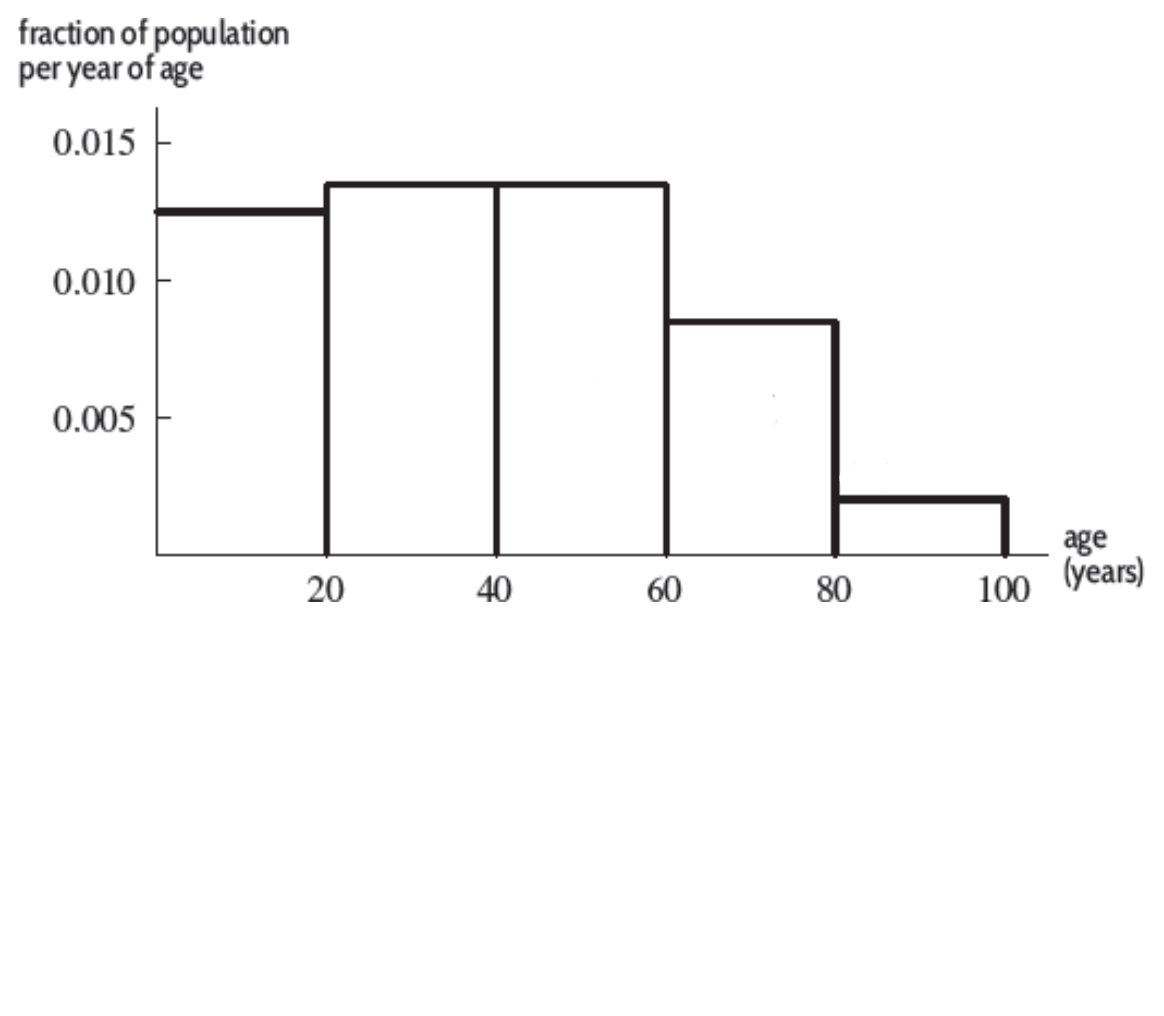
\includegraphics[scale=0.4]{fractiongraph}
    \end{center}

    \vspace{-3cm}
    
    \item Now consider the following new table of US age distribution, which is more refined. Let $Y$ be the new group number of a randomly selected person in the US. Sketch a histogram for the probability mass function of Y.

    \begin{table}[h!]
        \centering
        \begin{tabular}{c|c|c}
            \hline
           Group Number & Age Group & Percentage of Population \\
           \hline
            1 & 0-9 & 12\% \\
            2 & 10-19 & 13\% \\
            3 & 20-29 & 14\% \\
            4 & 30-39 & 13\%\\
            5 & 40-49 & 13\% \\
            6 & 50-59 & 14\% \\
            7 & 60-69 & 11\%\\
            8 & 70-79 & 6\% \\
            9 & 80-89 & 3\%\\
            10 & 90-99 & 1\% \\
           \hline
        \end{tabular}
    \end{table}

    \begin{center}
    \begin{tikzpicture}[scale=1]
          \begin{axis}[
            %xlabel={$x$},
            %grid = major,
            %xtick       = {1,2,3,4,5,6,7,8,9},
            %xticklabels = {$1$,$2$,$3$,$4$,$5$,$6$,$7$,$8$,$9$},
            %ytick       = {-3, -2, -1, 0,1,2,3,4},
            %yticklabels = {$-3$, $-2$, $-1$, $0$,$1$,$2$,$3$,$4$},
            ylabel={},
            axis lines = middle,
            ticks=none,
            xticklabel=\empty,
            yticklabel=\empty,
            domain      = -1:9.5,
            restrict y to domain=-3.5:2.5,
            xmin = 0, xmax = 10,
            ymin = 0, ymax = 4.5,
            height=2.1in, width=4in,
            %grid=both, grid style=dashed
          ]
          %\draw[ultra thick, red,--] (-2/3,1/3) -- (2,3) -- (3,3) -- (7, -3) -- (9.5, -0.5);
          %\node at (4,3) {$f(x)$};
          \end{axis}
    \end{tikzpicture}
    \end{center}


    \item Consider the corresponding fraction-of-population vs age graph. What does the area of each rectangle represent, and what mathematical concept in this course does this remind you of?

    \vfill
\end{enumerate}
    \newpage


\exercise{\bf\color{Orange}P1} 

You observe your friend tossing a coin. You saw them toss the coin twice and both times they got \emph{HEADS}. Do you think landing on \emph{TAILS} is more likely on the next toss?

\begin{enumerate}[label=(\alph*)]

\item  (Pre-Class Activity)
Assume the coin is fair, so each outcome in the sample space is equally likely. What is the sample space for first two flips? What does the probability mass function look like?

{\Large
    \[
    S = \rule[-8pt]{4in}{0.4pt}
    \]
}

\begin{table}[h!]
        \centering
        \begin{tabular}{|c|c|c|c|c|}
            \hline
           $x$  & \hspace{1.5cm} & \hspace{1.5cm} &\hspace{1.5cm}  & \hspace{1.5cm}  \\
           \hline
           $p(x)$  & \hspace{1.5cm} & \hspace{1.5cm} & \hspace{1.5cm}& \hspace{1.5cm} \\
           \hline
        \end{tabular}
\end{table}

\item 
Now suppose you observe that the first two tosses both landed on \emph{HEADS}. If the coin is fair and we flip once more, answer the following:  
\begin{enumerate}[label=\roman*.]
\item What is the new sample space for the next (third) toss?  
\vspace{2cm}
\item What are the probabilities of those outcomes?
\end{enumerate}
\vspace{2cm}

\item Reflect on whether or not observing “HH” in the first two tosses makes a tails outcome more likely in the third toss. Do you intuitively think ‘HHHHH’ is less random outcome than ‘HHTHT’?
\vfill

\end{enumerate}

\newpage

\exercise{P1}
Your best friend skipped class today  and only realized that probability is part of next Knowledge Checkpoint on the exam day. With almost no time to prepare, you want to highlight the core takeaways from today’s class. Suppose they’ve at least reviewed the pre-class. Which specific concepts or solving techniques from today should they focus on?

\newpage

\exercise{\bf\color{Orange}P1} Two fair six-sided dice are rolled and the result of each die is recorded. Below is a table of all possible outcomes.

\begin{center}
    
\includegraphics[scale=0.5]{Fall 2024/Lessons/jimLessons/lesson24_Review/images/sum2Dice.pdf}
\end{center}

\begin{enumerate}[label=(\alph*)]
    %\item What is the size of the sample space $S$ of this experiment?

    %\vfill

    \item Let $X$ be the sum of the two resulting numbers. Write down the probability mass function for the random variable $X$ and sketch its histogram.

    \vfill\vfill\vfill

    \item Find $P(X\ge 9)$.

    \vfill\vfill

    \item Find $P(X\text{ is a multiple of 3})$.

    \vfill\vfill
\end{enumerate}





%%%%%%%%%
\newpage%
%%%%%%%%%

{\bf\color{blue} Extra Practice 1.} \reversemarginpar\marginnote{\fbox{\bf\color{Orange} P1}}  A standard 6-sided die has been painted so that it has 2 {\color{red}red} sides, 2 {\color{ForestGreen}green} sides, and 2 {\color{blue}blue} sides.

\begin{itemize}
    \item[(a)] In an experiment where the die is rolled and the color of the upturned face is recorded, what is the sample space $S$?

    {\Large
    \[
    S = \rule[-8pt]{4in}{0.4pt}
    \]
    }
    
    \item[(b)] In an experiment where the die is rolled twice and the color of the upturned face is recorded each time, what is the sample space $S$?

    {\Large
    \[
    S = \rule[-8pt]{4in}{0.4pt}
    \]
    }
    
\end{itemize}

{\bf\color{blue}Extra Practice 2.}\reversemarginpar\marginnote{\fbox{\bf\color{Orange} P1}} 
The World Series is the annual championship series of Major League Baseball. Currently, its format is a direct competition between two teams of up to seven games, where the first team wins four games wins the championship.

For example, if team A wins the first 3 games, team B wins the 4th game, and team A wins the 5th game, then team A wins the series. Game 6 and Game 7 will then not be played since a winner has already been determined. In this case, it took 5 games to determine the winner.

    \begin{itemize}
    \item[(a)] Let $X$ represent the number of games it takes to determine the winner of the World Series. What are all possible values of $X$?
    \vfill

    \item[(b)] Suppose team A won the first 2 games and team B won the third. For each of the remaining four games, assume each team has an equal chance of winning. 

    Find $P(X\le 5)$.

    \vfill

    \end{itemize}
\end{document}